\section{Bayesian Inference}

\subsection*{Bayes Filter}\begin{frame}\frametitle{Bayes Filter}
    \begin{itemize}
        \item Bayesian filtering is one of the most effective techniques to effectively manages noise.
        \pause
        \item The Bayes filter is sequential algorithm with two steps:
        \begin{itemize}
            \item \textbf{Predict:} Based on motion model and previous posterior, calculate the next state:
                \begin{equation*}
                    p\left(\vecat{x}{k} | \vecat{z}{1: k-1}\right) = \int
                        \underbrace{p\left( \vecat{x}{k} | \vecat{x}{k-1} \right)}_{\text{motion model}}
                        \quad
                        \underbrace{p\left( \vecat{x}{k-1} | \vecat{z}{1: k-1} \right)}_{\text{posterior at } k-1}
                        \mathrm{d} \vecat{x}{k-1}.
                \end{equation*}
            \pause
            \item \textbf{Update:} Revise the state estimate based on the measurement model and predicted density:
                \begin{equation*}
                    p\left(\vecat{x}{k} | \vecat{z}{1: k}\right) \propto
                    \underbrace{p\left(\vecat{z}{k} | \vecat{x}{k}\right)}_{\text{measurement model}}
                    \quad
                    \underbrace{p\left(\vecat{x}{k} | \vecat{z}{1: k-1}\right)}_{\text{predicted density}}.
                \end{equation*}
        \end{itemize}
        \pause
        \item For a \textit{single target} with Gaussian-linear dynamics, use the Kalman filter.
    \end{itemize}
\end{frame}

\subsection*{Multi-Target Tracking}\begin{frame}\frametitle{Multi-Target Tracking}
    \begin{itemize}
        \item Recall the target-to-measurement assignment problem.
        \begin{onlyenv}<1>
        \begin{center}
            \vspace{1em}
            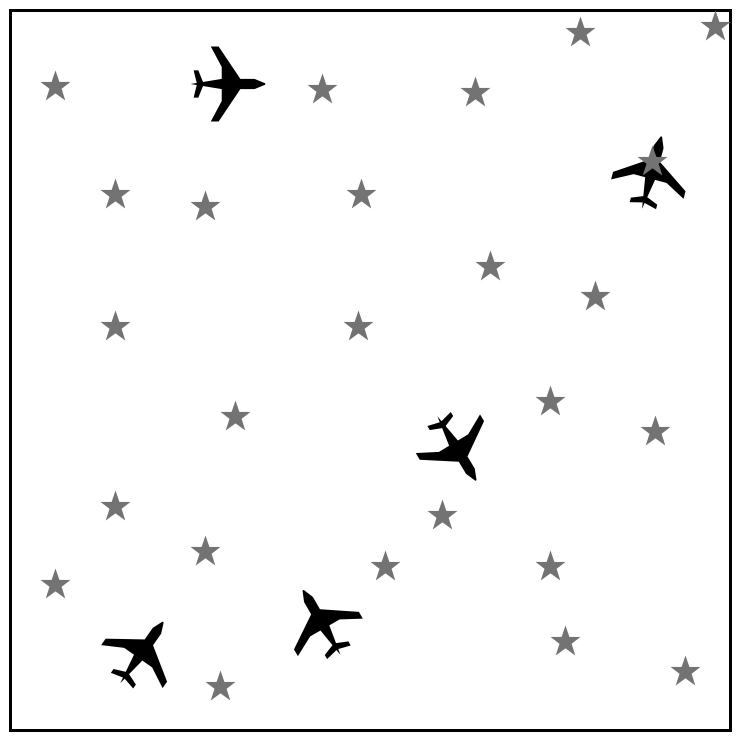
\includegraphics[width=0.4\linewidth]{pic/assignment-problem-gray.png}
        \end{center}
        \end{onlyenv}
        \pause
        \item Here, \textit{all} assignments have a certain likelihood.
        \pause
        \item Each assignment is a \textit{hypothesis}, and each likelihood is its \textit{weight}.
        \pause
        \item Number of hypotheses can increase exponentially. All possibilities should be considered, as it's unclear which ones are correct.
        \pause
        \item Posterior normalization calculation? \pause \alert{Approximations needed!}
        \pause
        \item Or, consider a different strategy...
    \end{itemize}
\end{frame}
